Общая схема суперкомпилятора представлена на рисунке~\ref{fig:scompScheme}.

\begin{figure}[h!]
\center
\includegraphics[scale=0.76]{Kuklina/src/review/scompflow.pdf}
\caption{Общая схема суперкомпилятора.}
\label{fig:scompScheme}
\end{figure}

История вычислений при суперкомпиляции представляется в виде \emph{графа процессов} --- корневого ориентированного графа,
в котором каждая ветвь --- это отдельный путь вычислений, а каждый узел --- состояние системы или \emph{конфигурация}.
Конфигурация обобщённо описывает множество состояний вычислительной системы или её подсистемы.
К примеру, конфигурацией можно назвать выражение $1 + x$, в котором параметр $x$ пробегает
все возможные значения своего домена (допустим, множество натуральных чисел) и задаёт
таким образом множество состояний программы~\cite{turchinSC}.

% Процесс построения графа процессов называется \emph{прогонкой} \origin{driving}.
\emph{Прогонкой}~\origin{driving} называется процесс построения графа процессов.
Во время прогонки производится шаг символьных вычислений, после которого
в граф процессов добавляются порождённые конфигурации; множество конфигураций
появляется тогда, когда ветвления в программе зависят от свободных переменных.
В данной работе шаг символьного вычисления именуется \emph{развёрткой}.

В процессе прогонки в конфигурациях могут появляться новые свободные переменные,
которые строятся из исходной конфигурации:
если при вычислении выражения его переменная перешла в другую переменную (к примеру, из-за сопоставления с образцом),
то в итоговую конфигурацию будет подставлена новая переменная и связь старой и новой сохранится в
некоторой \emph{подстановке}.
Подстановка --- это отображение из множества переменных в множество возможно замкнутых термов.
Применение подстановки к выражению заменит все вхождения переменных, принадлежащих её домену,
на соответствующие термы. %\todo{Что-нибудь ещё}

Пример графа процессов представлен на рисунке~\ref{fig:pgraphExample}.
\begin{figure}[h!]
\center
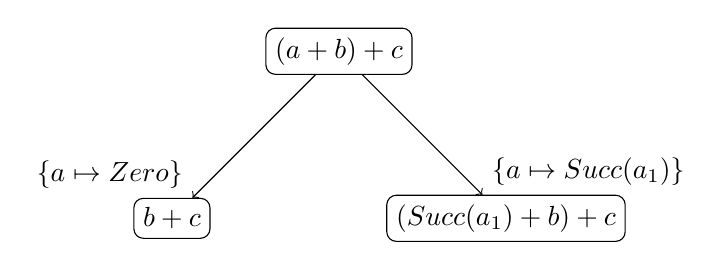
\begin{tikzpicture}[->,node distance=3cm, sibling distance=5cm]

  \tikzstyle{conf}=[rectangle,draw, rounded corners=.8ex]

  \node[conf] (root) {$(a + b) + c$} ;
  \node[conf] (childLeft) [below left of = root] {$b + c$};
  \node[conf] (childRight)[below right of = root] {$(\text{Succ}(a_1) + b) + c$};
  \path (root) edge node[above left,pos=1] {$\{a \mapsto \text{Zero}\}$} (childLeft)
        (root) edge node[above right,pos=1]{$\{a \mapsto \text{Succ}(a_1)\}$}(childRight);
\end{tikzpicture}

\caption{Пример части графа процессов.}
\label{fig:pgraphExample}
\end{figure}
Здесь при исполнении выражения $(a + b) + c$, где $a, b, c$ -- натуральные числа,
были рассмотрены возможные значения $a$: либо оно равно нулю (конструктор Zero), либо это некоторое
число $a_1$, которому прибавили единицу (конструктор Succ). Эти два случая могут задавать
различные пути исполнения и, соответственно, добавлены в дерево процессов как два различных состояния,
в одно из которых войдёт программа при исполнении.

Процесс прогонки может быть бесконечным, к примеру, когда происходят рекурсивные вызовы.
Для превращения бесконечного дерева вычисления в конечный объект, по которому можно
восстановить исходное дерево, используется \emph{свёртка.}

Свёртка~\origin{folding}~--- это процесс преобразования дерева процессов в граф, при котором
из вершины $v_c$ добавляется ребро в родительскую вершину $v_p$,
если выражение в конфигурации в $v_c$ и в $v_p$ равны с точностью до переименования.
Пример ситуации для свёртки изображён на рисунке~\ref{fig:pgraphFoldingExample},
на котором свёрточное ребро изображено пунктиром.

\begin{figure}[h!]
\center
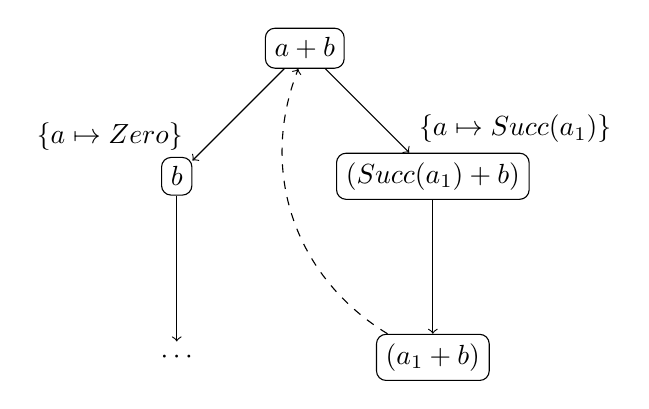
\begin{tikzpicture}[->,node distance=2.3cm, sibling distance=5cm]

  \tikzstyle{conf}=[rectangle,draw, rounded corners=.8ex]

  \node[conf] (root) {$a + b$} ;
  \node[conf] (childLeft) [below left of = root] {$b$};
  \node[conf] (childRight)[below right of = root] {$(\text{Succ}(a_1) + b)$};
  \node[conf] (childRight2)[below  of = childRight] {$(a_1 + b)$};
  \node (left)[below of = childLeft] {$\cdots$};

  \path (root) edge node[above left,pos=1] {$\{a \mapsto \text{Zero}\}$} (childLeft)
        (root) edge node[above right,pos=1]{$\{a \mapsto \text{Succ}(a_1)\}$}(childRight)
        (childLeft) edge (left)
        (childRight) edge (childRight2)
        (childRight2) edge[bend left=40, dashed] (root);
  %\draw[->] (childRight) to (childRight2);
  %\draw[->,dashed] (childRight2) to[bend left=90] (root);
\end{tikzpicture}

\caption{Пример свёртки.}
\label{fig:pgraphFoldingExample}
\end{figure}

Однако существуют ситуации, при которых свёртка не приведёт к тому, что граф превратится в
конечный объект. Такое может произойти, к примеру, когда два выражения структурно
схожи, но не существует переименования, уравнивающих их.

Для решения этой проблемы используется \emph{обобщение}~\cite{scGen}. Обобщение --- это процесс
замены одной конфигурации на другую, более абстрактную, описывающую больше состояний
программы. Для обнаружения ``похожей'' конфигурации используется предикат,
традиционно называемый \emph{свистком}:
% свисток пробегает по всем родителям текущей конфигурации и
свисток определяет, похожа ли конфигурация на кого-то из родителей текущей конфигурации.
В случае, когда свисток сигнализирует о найденной схожести, применяется обобщение.
Сам шаг обобщения может произвести действия двух видов:
\begin{itemize}
\item \emph{обобщение вниз} приводит к тому, что новая конфигурация заменяет текущую в графе процессов;
%\item \emph{обобщение вверх} приводит к замене родительской конфигурации на обобщённую;
\item \emph{разделение}~\origin{split} используется для декомпозиции выражения, элементы которого затем
будут обработаны отдельно.
\end{itemize}
Пример обобщения представлен на рисунке~\ref{fig:pgraphGenExample}
\begin{figure}[h!]
\center
\begin{tikzpicture}[->,node distance=2.5cm, sibling distance=5cm]
  \tikzstyle{conf}=[rectangle,draw, rounded corners=.8ex]
  \node[conf] (root) {$a \times b$};
  \node[conf] (childLeft)[below left of = root] {Zero};
  \node[conf, very thick] (childRight)[below right of = root] {$(a_1 \times b) + b$};
  \node[conf, text width = 2.5cm, thick, dashed] (childGen)[below of = childRight] {$v_1 + v_2$, $v_1 := b$, $v_2 := a_1 \times b$};
  \node[conf] (childGenLeft)[below left of = childGen] {$v_1 + v_2$};
  \node[conf] (childGenRight)[below right of = childGen] {$a_1 \times b$};

  \path (root) edge node[above left,pos=1] {$\{a \mapsto \text{Zero}\}$} (childLeft)
        (root) edge node[above right,pos=1]{$\{a \mapsto \text{Succ}(a_1)\}$}(childRight)
        (childRight) edge (childGen)
        (childGen) edge (childGenLeft)
        (childGen) edge (childGenRight)
        % (childGenRight) edge[bend right=90, dashed] (root)
  ;

 \draw[->, dashed] (childGenRight) to[out=20,in=10,looseness=1.9] (root);

\end{tikzpicture}

% \includegraphics[scale=0.3]{./review/scgenex_temp.png}

\caption{Пример обобщения.}
\label{fig:pgraphGenExample}
\end{figure}

Построение программы по графу конфигураций называется \emph{резидуализацией}, а
построенная программа --- \emph{остаточной} \origin{residual}.
Алгоритм выявления остаточной программы основан на обходе дерева, но
в остальном полностью зависит от языка.
